\chapter{Introduction}
\label{ch1}

\adjustmtc % Adjust Minitoc to right chapter
%%%%%%%%%%%%%%%%%%%%%%%%%%%%%%%%%%%%%%%
% IMPORTANT
\singlespacing % THESE THREE
\minitoc % LINES MUST APPEAR IN
\doublespacing % EVERY CHAPTER
% COPY THEM IN ANY NEW CHAPTER
%%%%%%%%%%%%%%%%%%%%%%%%%%%%%%%%%%%%%%%


\section{Project Introduction}
This project presents general framework for Algorithmic trading native to Julia, capable of solving portfolio optimization problems using \ac{MPC}, called AirBorne. 

In particular, in Chapter \ref{ch5}, AirBorne will be used as the simulation framework running a state of the art \ac{MPC} that uses \ac{HMM} in combination with a Mean-Variance framework to estimate an optimal portfolio distribution over time that maximizes a balance between expected returns and the variance of the return.

In Chapter \ref{ch1} and introduction to the project, its motivation and related works are addressed. Chapter \ref{ch2} introduces necessary concepts for Financial modelling that be linked to the dynamics of the system.  Chapter \ref{ch3} addresses the \ac{OCP} formulation and introduces the \ac{MPC} model.  Chapter \ref{ch4} addresses the design of AirBorne and identifies some unique traits of the Julia language leveraged on the project. Lastly Chapter \ref{ch5} presents results of the implementation of multiple trading strategies using AirBorne as the framework for the simulations.

\subsection{Motivation}

Portfolio optimization and algorithmic trading is an active area of research in all fields from mathematical formulations \cite{RL2022,2022OptimalControl} to ethics and law  \cite{ethicsAndLaw2022}, whilst some algorithms are reported to outperform human traders on normal circumstances on complex market conditions humans still have the edge \cite{algorithmicTradingWithHumanTraders}. In recent years control theory techniques such as \ac{MPC} are being increasingly used for portfolio optimization, formulating the management of assets as a control problem \cite{MultiPeriod_PO_mpc}. 

At the same time Julia, a relatively new language, often compared to Python on its expressiveness and C on its performance, lacks well developed and maintained packages suitable for algorithmic trading and backtesting hindering its potential and adoption rate for algorithmic trading purposes \cite{juliaReview2021}. 

Therefore the aim of this project is to produce software native to Julia for portfolio optimization and algorithmic trading simulation to accelerate research in the future in the area and this language. 

\subsection{Related work}

Many groups in Github have tried to deploy similar software in the past, most of the attempts resulted in projects with great initial development but died out eventually due to lack of continuous support and maintenance. Some of the most prominent related projects are:

\begin{enumerate}
    \item \textbf{JuliaQuant:} They tried to provide an ecosystem of algorithmic trading tools from analysis to model of portfolios. Although they have been around for more than 5 years the intensity of development has winded down significantly, having their last commit to any of their repositories to January 2023, \url{https://github.com/JuliaQuant}. 
    \item \textbf{Julia Finance:} Also following a similar approach to JuliaQuant they provided different models of entities such like assets and currencies. Most of the repositories are not actively maintained with the exception of ``BusinessDays", \url{https://github.com/JuliaFinance}.
    \item \textbf{Trading.jl:} This is a single package focused on designing tools for back-testing, is a relatively young package and although promising it being supported by a single person poses a key-person risk.\url{https://github.com/louisponet/Trading.jl}
\end{enumerate}

All these previous attempts have in common to be maintained by a handful of individuals, with a sharp fast initial development and subsequent slower development pace. 

AirBorne has the advantage of being institutionally backed by Imperial College London, ensuring its support and maintenance as long as the project is deemed relevant by their leaders, this ensures renewal of people for its support and continuous improvement until it has features rich enough for the community to adopt it and evolve into a community maintained open-source package.

This approach similar to python starts the package being institutionally backed on its early stages were continuous support and improvement are critical for the development of the package until is of enough value for the community to adopt, nourish and maintain, such as the Python and C++ AirBorne counterparts Zipline and Zorro projects.


\subsubsection{Julia package ecosystem}
In Julia is important to design software packages compatible with other related and used packages, which is commonly known as the ecosystem of a package. Some of the packages AirBorne's ecosystem are:
\begin{enumerate}
    \item \textbf{ValueAtRisk.jl:} Package specialized in calculated the \ac{VaR} metric.
    \item \textbf{Currencies.jl:} Alternative package for currency modelling complying with ISO guidelines.
    \item \textbf{ARCHModels.jl:} Produces ARCH models. ARCH models are variants of ARMAX models widely used in financial applications such as inflation simulation with seasonal volatility \cite{ARCHModels.jl,Periodic_ARCHModels_og_paper,ARCHModels_og_paper}.
    \item \textbf{DirectSearch.jl: } A package developed by Imperial College London, which implements the optimization algorithm \ac{MADS}\cite{DirectSearch.jl,MADS_og_paper_06}. It  derivative free optimization algorithm, ideal for empirically driven optimization problems where a descent direction may not be available or hard to deduce.
\end{enumerate}

\subsubsection{Past research projects}

In recent years Imperial students have tried many formulations to address advisory algorithmic trading, were a computer suggest trading strategies to a human prior to execution. Some techniques used were Reinforcement Learning  \cite{RLMasoud2021}, Behavioural Control Theory  \cite{BCTScott2022,BCTKhaliq2022} and Data Enabled Predictive Control \cite{DeePCMohamed2023}.

Although many of these projects achieved a stand alone implementation of portfolio optimization they didn't produce a general software capable of implementing custom trading strategies and be able to compare and analyze them. 

This project will build on top of their work and create a generalized framework to benchmark and compare different techniques for portfolio optimization in the Julia programming language along with an implementation using Optimal Control.


\section{Introduction AirBorne}
Chapter \ref{ch2} introduces the theoretical background for the algorithmic trading problem but also establishes some links between the theory and the design of the software. Therefore an overall introduction to the \ac{HLD} of AirBorne will be presented here and justified through Chapters \ref{ch2} and \ref{ch4}.

\begin{figure}[h!]
    \centering
    % \includesvg[width=1\textwidth]{imgs/ch1/SoftwareArchitecture.svg}
    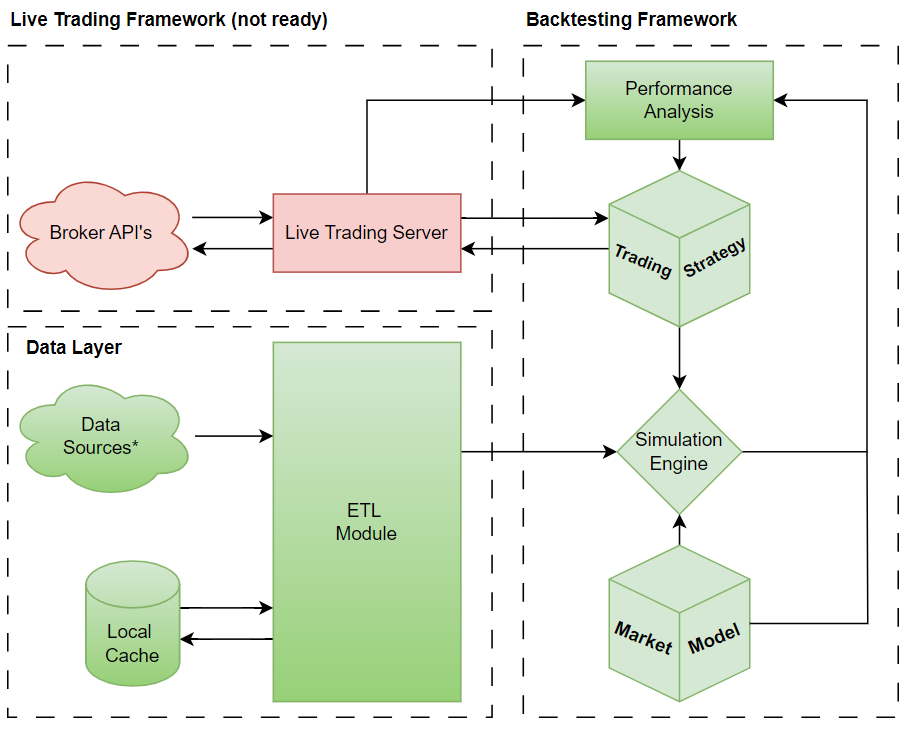
\includegraphics[width=1\textwidth]{imgs/ch1/architecture.png}
    \caption[AirBorne: Overall Architecture]{AirBorne: Overall Architecture}
    \label{fig::AirBorneArchitecture}
\end{figure}

Figure \ref{fig::AirBorneArchitecture} shows the overall architecture of AirBorne, which is composed of three components:
\begin{enumerate}
    \item \textbf{Data Layer:} Where connections to data sources, local storage in persisted memory (the cache) and common data manipulation take place.
    \item \textbf{Backtesting Framework:} Where simulations take place and trading strategies, models for markets and performance calculations are defined.
    \item \textbf{Live Trading Framework:} This layer provides an interface with brokerage accounts and broker \ac{API}s, allowing to switch a trading strategy from simulation to live or paper trading seamlessly. 
\end{enumerate}

Of these three components, for the project the Backtesting Framework and Data Layer were developed, and the implementation of the Live Trading Framework was left out from the scope of the project.

Figure \ref{fig::AirBorneModules} shows the hierarchy of submodules, where the higher submodules have some dependency or are supported by the lower ones.

\begin{figure}[h!]
    \centering
    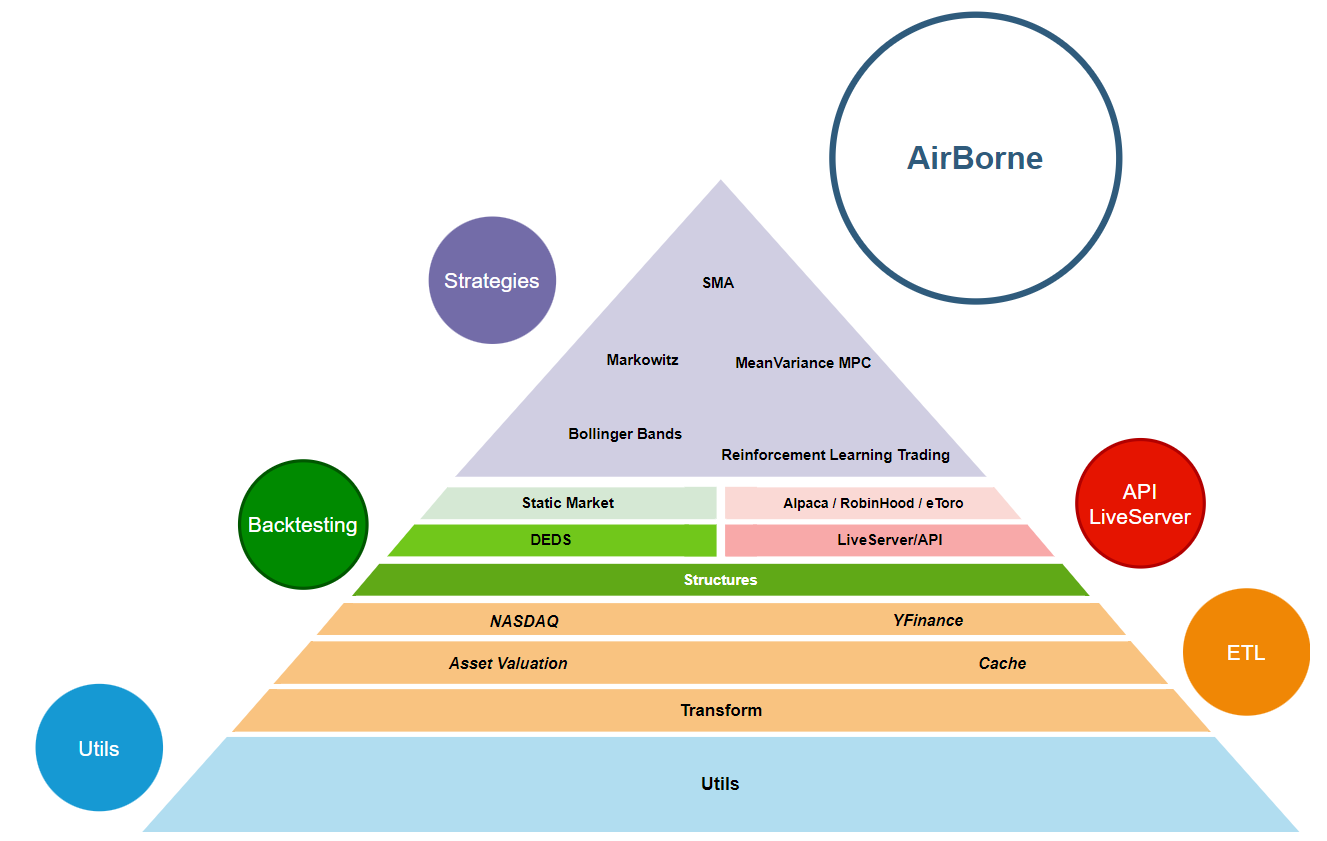
\includegraphics[width=1\textwidth]{imgs/ch1/Hierarchy.png}
    \caption[AirBorne: Module Hierarchy]{AirBorne: Module Hierarchy}
    \label{fig::AirBorneModules}
\end{figure}

\textbf{Utils} contains basic functions used throughout the module, this reduces duplicate code throughout, \textbf{ETL} provides the tools for data handling and storage of data in the system that can be processed during the simulation or backtesting stages. Then the pyramid branches into \textbf{Backtesting} and \textbf{Live Trading}, both of this layers share common data structures, but one specializes in simulation/modelling of the market whilst the second one provides direct connection to the real market. Lastly \textbf{Strategies} produces investment strategies that are designed to be incorporated either on backtesting or live-trading instances.


\section{Notation}

Standard notation has been adopted in the Thesis, most of which is defined in this section and used throughout the remainder of the Thesis. When new notation, not included in this section is introduced, this is defined in the relevant parts of the Thesis.\smallskip\\

\begin{enumerate}
    \item $\delta_{\odot}$: Delta Kronecker applied to each entry of an array
    \item $\odot$: Element wise product
\end{enumerate}

% \indent The symbol $\mathbb{R}_{\ge0}$ ($\mathbb{R}_{>0}$) denotes the set of non-negative (positive) real numbers; $\mathbb{C}_{<0}$ denotes the set of complex numbers with strictly negative real part; $\mathbb{C}_{0}$ denotes the set of complex numbers with zero real part and $\mathbb{D}_{<1}$ the set of complex numbers with modulo less than one.\smallskip\\
% \indent The symbol $I$ denotes the identity matrix and $\sigma(A)$ denotes the spectrum of the matrix $A\in\mathbb{R}^{n\times n}$. The symbol $\otimes$ indicates the Kronecker product and $||A||$ indicates the induced Euclidean matrix norm. Given a list of $n$ elements $a_i$, $\diag(a_i)$ indicates a diagonal matrix with diagonal elements equal to the $a_i$'s. The vectorization of a matrix $A\in\mathbb{R}^{n\times m}$, denoted by $\vect(A)$, is the $nm \times 1$ vector obtained by stacking the columns of the matrix $A$ one on top of the other, namely $\vect(A)=[a_1^{\top},a_2^{\top},\dots,a_m^{\top}]^{\top}$, where $a_i\in\mathbb{R}^n$ are the columns of $A$ and the superscript $\top$ denotes the transposition operator. The superscript $*$ indicates the conjugate transpose operator.\smallskip\\
% \indent The symbol $\Re[z]$ indicates the real part of the complex number $z$, $\Im[z]$ denotes its imaginary part and $\iota$ denotes the imaginary unit. The symbol $\epsilon_k$ indicates a vector with the $k$-th element equal to 1 and with all the other elements equal to 0. Given a function $f$, $\overline{F}$ represents its phasor at $\omega$, whereas $<\!f(t)\!>$ indicates its time average.\smallskip\\
% \indent Given a set of delays $\{\tau_j\}$, the symbol $\mathfrak{R}_T^n=\mathfrak{R}_T^n([-T,0],\mathbb{R}^n)$, with $T=  \max_j\{\tau_j\}$, indicates the set of continuous functions mapping the interval $[-T,0]$ into $\mathbb{R}^n$ with the topology of uniform convergence . The subscripts ``$\tau_j$'' and ``$\chi_j$'' denote the translation operator, \textit{e.g.}\ $x_{\tau_j}(t)=x(t-\tau_j)$.\smallskip\\
% \indent Let $\bar s \in \mathbb{C}$ and $A(s)\in \mathbb{C}^{n \times n}$. Then $\bar s\notin\sigma(A(s))$ means that $\det(\bar s I-A(\bar s ))\ne0$. $\sigma(A(s))\subset\mathbb{C}_{<0}$ means that for all $\bar s$ such that $\det(\bar s I-A(\bar s ))=0$, $\bar s \in\mathbb{C}_{<0}$.\smallskip\\
% \indent The symbol $\mathcal{L}(f(t))$ denotes the Laplace transform of the function $f(t)$ (provided that $f(t)$ is Laplace transformable) and $\mathcal{L}^{-1}\{F(s)\}$ denotes the inverse Laplace transform of $F(s)$ (provided it exists). With some abuse of notation, $\sigma(\mathcal{L}(f(t)))$ denotes the set of poles of $\mathcal{L}(f(t))$. Given two functions, $f:Y\to Z$ and $g:X\to Y$, with $f\,\circ\,g:X\to Z$ we denote the composite function $(f\,\circ\,g)(x)=f(g(x))$ which maps all $x\in X$ to $f(g(x))\in Z$.

